\documentclass[tikz,border=5pt]{standalone}
\usepackage[UTF8]{ctex}
\usepackage{amsmath,amssymb}
\usetikzlibrary{arrows.meta,calc,angles,quotes,patterns,decorations.pathmorphing}
\definecolor{field}{HTML}{176B9B}
\definecolor{force}{HTML}{B64B32}
\tikzset{>=Latex,line width=.8pt,every node/.style={font=\small},field/.style={color=field},force/.style={color=force},body/.style={draw=black,fill=blue!5},ghost/.style={dashed,gray},labelbox/.style={fill=white,inner sep=1.2pt}}
\begin{document}
\begin{tikzpicture}[scale=2]
\draw[thick](-.1,0)--(2.1,0);
\fill[gray!10](0,0)--(0,1)--(1,0)--cycle;
\draw[thick](0,0)--(0,1)--(1,0);
\draw[thick](-.05,1.45)--(1.1,1.45);
\fill(.3,1.43)circle(1.3pt);\draw[->](.3,1.37)--(.3,1.05);
\draw[<->](-.25,0)--(-.25,1)node[midway,left]{$h$};
\draw[<->](0,-.22)--(1,-.22)node[midway,below]{$h$};
\draw[<->](1.35,0)--(1.35,1.45)node[midway,right]{$\lambda h$};
\draw[ghost,domain=0:1.183216,samples=51]plot({.3+1.224745*\x},{.7-.5*\x*\x});
\node[below right]at(1,0){底端};
\end{tikzpicture}
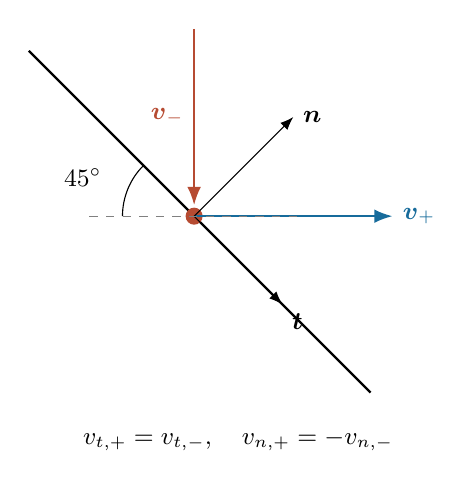
\begin{tikzpicture}[scale=1.4]
\draw[thick](-1.5,1.5)--(1.6,-1.6);
\fill[force](0,0)circle(2.2pt);
\draw[force,->,thick](0,1.7)--(0,.1)node[midway,left]{$\boldsymbol v_-$};
\draw[field,->,thick](0,0)--(1.8,0)node[right]{$\boldsymbol v_+$};
\draw[->](0,0)--(.9,.9)node[right]{$\boldsymbol n$};
\draw[->](0,0)--(.8,-.8)node[below right]{$\boldsymbol t$};
\draw[ghost](-.95,0)--(.95,0);
\draw(-.65,0)arc(180:135:.65);
\node[left]at(-.75,.35){$45^\circ$};
\node[below]at(.4,-1.85){$v_{t,+}=v_{t,-},\quad v_{n,+}=-v_{n,-}$};
\end{tikzpicture}
\begin{tikzpicture}
\begin{scope}[scale=2.4]
\draw[thick](-.05,0)--(1.5,0);
\draw[thick](0,0)--(0,1)--(1,0);
\draw[field,thick,domain=0:1.0583,samples=50]plot({.04+.52915*\x},{.96-.5*\x*\x});
\fill[force](.6,.4)circle(2pt)node[right]{$x_2<h$};
\draw[->](.04,1.2)--(.04,.98);
\node[above]at(.65,1.3){$\lambda=1.1,\ y=0.96h$};
\end{scope}
\begin{scope}[xshift=5cm,scale=2.4]
\draw[thick](-.05,0)--(1.5,0);
\draw[thick](0,0)--(0,1)--(1,0);
\draw[ghost](1,0)--(1.2,-.2);
\draw[field,thick,domain=0:1.4071,samples=50]plot({.01+.72111*\x},{.99-.5*\x*\x});
\draw[ghost,domain=1.4071:1.4422,samples=8]plot({.01+.72111*\x},{.99-.5*\x*\x});
\fill[force](1.05,-.05)circle(2pt);
\draw[force] (1.05,-.05)--(1.3,-.3)node[right]{延拓交点};
\node[above]at(.65,1.3){$\lambda=1.25,\ y=0.99h$};
\end{scope}
\end{tikzpicture}
\begin{tikzpicture}[scale=3]
\draw[thick](-.05,0)--(1.8,0);
\draw[thick](0,0)--(0,1)--(1,0);
\draw[ghost](-.03,1.25)--(1.15,1.25)node[right]{$H=5h/4$};
\draw[field,thick,domain=0:1.4071,samples=60]plot({.01+.72111*\x},{.99-.5*\x*\x});
\draw[force,thick,domain=0:.1732,samples=30]plot({.985+1.57162*\x},{.015-.5*\x*\x});
\fill(1,0)circle(1.5pt)node[below left]{$h$};
\fill[field](1.02468,0)circle(1.5pt);
\draw[<->](1,-.2)--(1.25722,-.2)node[midway,below]{$\Delta$};
\draw[ghost](1.25722,0)--(1.25722,-.2);
\node[above right]at(.4,.87){$y\to h^-$};
\node[force,above]at(1.2,.15){$y\to0^+$};
\node[below]at(.8,-.55){两个端点极限均有 $\Delta\to0$};
\end{tikzpicture}
\end{document}
